\title{Question 6}
\author{Anshika Raman \\ Roll No: 210050014
    \and Kushal Aggarwal \\ Roll No: 210100087
    \and Kavan Vavadiya \\ Roll No: 210100166}


\documentclass[11pt]{article}
\usepackage{graphicx, caption}
\usepackage{amsmath}
\usepackage{amssymb}
\usepackage{hyperref}
\usepackage{ulem}
\usepackage[margin=0.5in]{geometry}
\begin{document}
\maketitle
\begin{enumerate}
\item[Que 6.]
\begin{enumerate}

\item[(b)] \
The resulting affine transformation from the set of points chosen is the following.
\begin{equation}
    \textit{affine}=\begin{bmatrix}
        1.0565 & 0.0011 & 25.1935\\
-0.0146 & 1.0111 & 21.2181\\
0 & 0 & 1
    \end{bmatrix}
\end{equation}
\item[(c)] \
The following are the results from the nearest neighbour interpolation.
\begin{figure}[!htb]
\centering
\minipage{0.5\textwidth}
  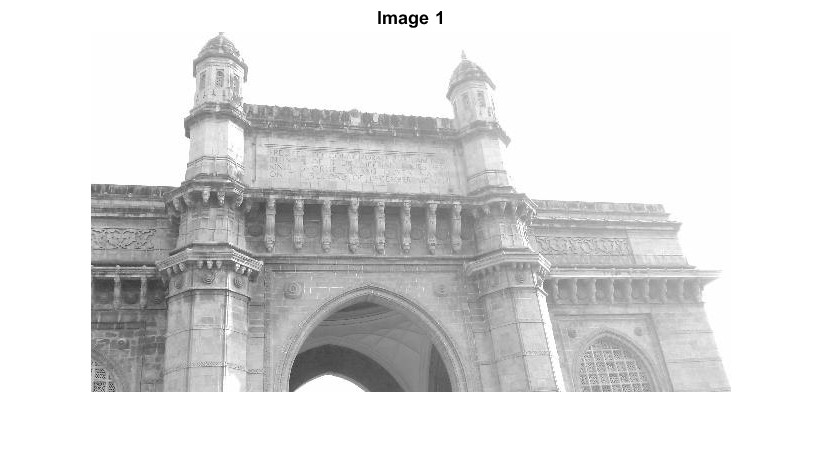
\includegraphics[width=9cm]{../images/Im1.jpg}
  \endminipage\hfill
  \minipage{0.5\textwidth}
 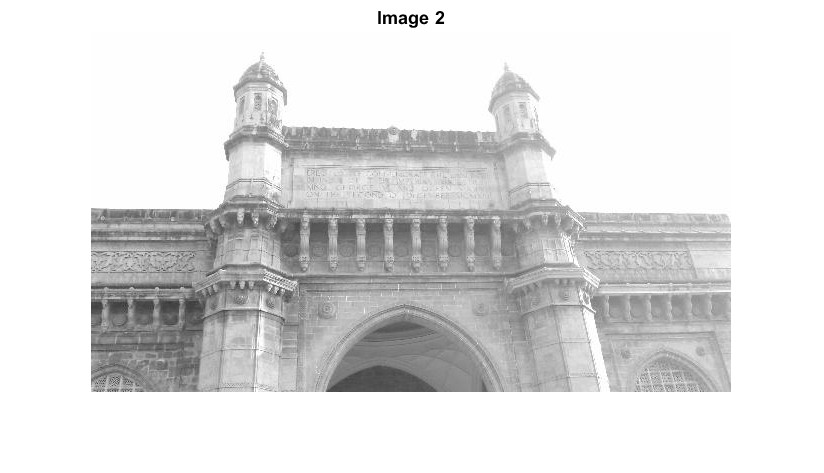
\includegraphics[width=9cm]{../images/Im2.jpg}
    \endminipage\hfill
  \minipage{0.5\textwidth}
  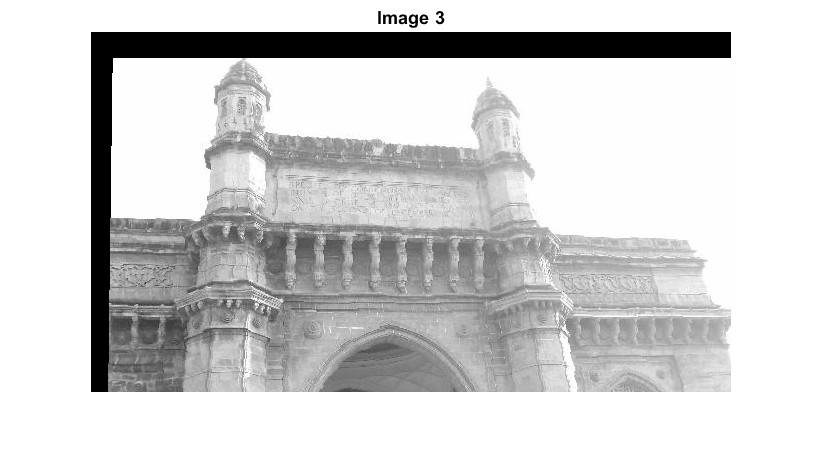
\includegraphics[width=9cm]{../images/nearest.jpg}
  \endminipage\hfill
\caption{Nearest neighbour interpolation}
\end{figure}

\pagebreak
\item[(d)] \
The following are the results from the bolinear interpolation.
\begin{figure}[!htb]
\centering
\minipage{0.5\textwidth}
  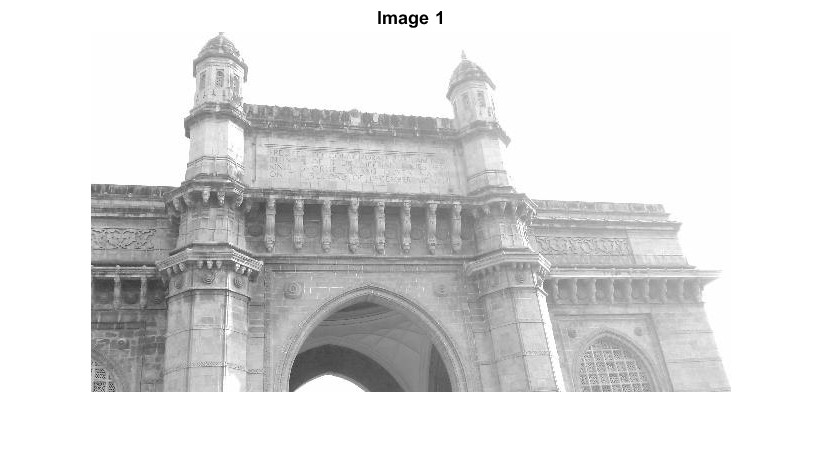
\includegraphics[width=9cm]{../images/Im1.jpg}
  \endminipage\hfill
  \minipage{0.5\textwidth}
 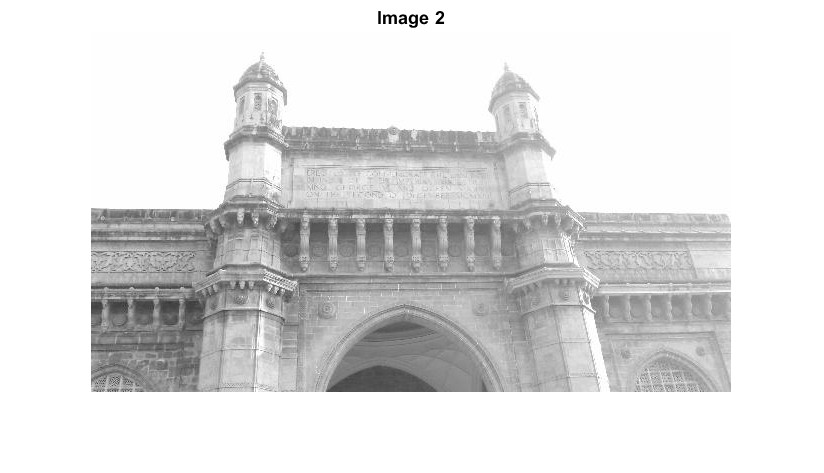
\includegraphics[width=9cm]{../images/Im2.jpg}
    \endminipage\hfill
  \minipage{0.5\textwidth}
  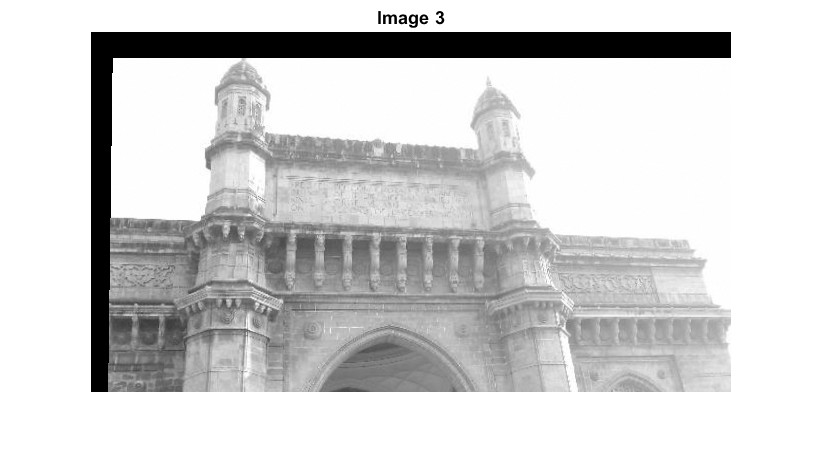
\includegraphics[width=9cm]{../images/bilinear.jpg}
  \endminipage\hfill
\caption{Bilinear interpolation}
\end{figure}

\item[(e)] \
If the points chosen are collinear, the pseduo inverse will not exist and small variations in selecting collinear points will result in large unwanted distortions in an image created from the affine matrix. 
\end{enumerate}
\end{enumerate}
\end{document}